\graphicspath{
  {./images/bmps/}{./images/vects/}{./images/}
  {./images/presentation/bmps/}{./images/presentation/vects/}{./images/presentation/}
  {./images/chapter00/bmps/}{./images/chapter00/vects/}{./images/chapter00/}
  {./images/chapter01/bmps/}{./images/chapter01/vects/}{./images/chapter01/}
}

\subsection{Change Detection for Obstacle Localization in Images}
\begin{frame}{Pipeline}
  \begin{center}
    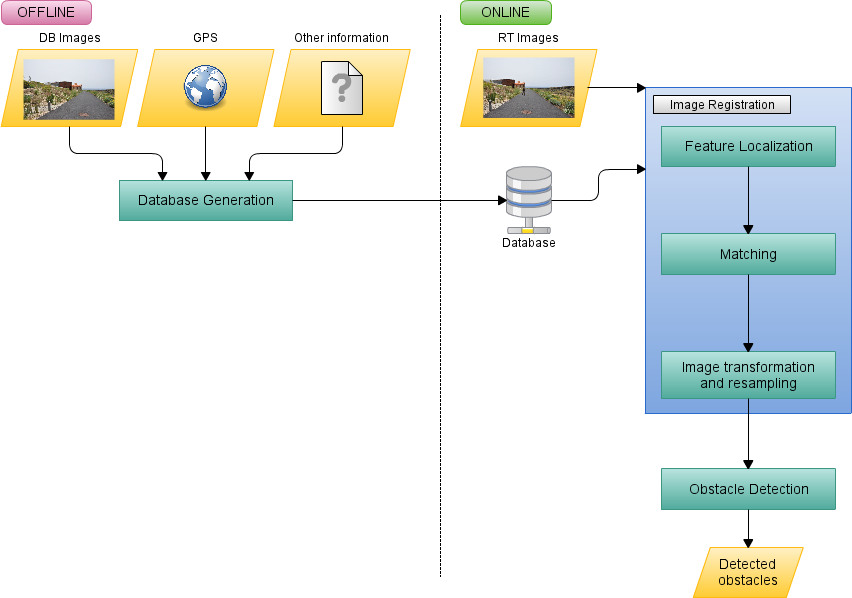
\includegraphics{pipeline_cp01}
  \end{center}
  
  \note {
  }
\end{frame}

\begin{frame}{Database generation}
  \begin{center}
    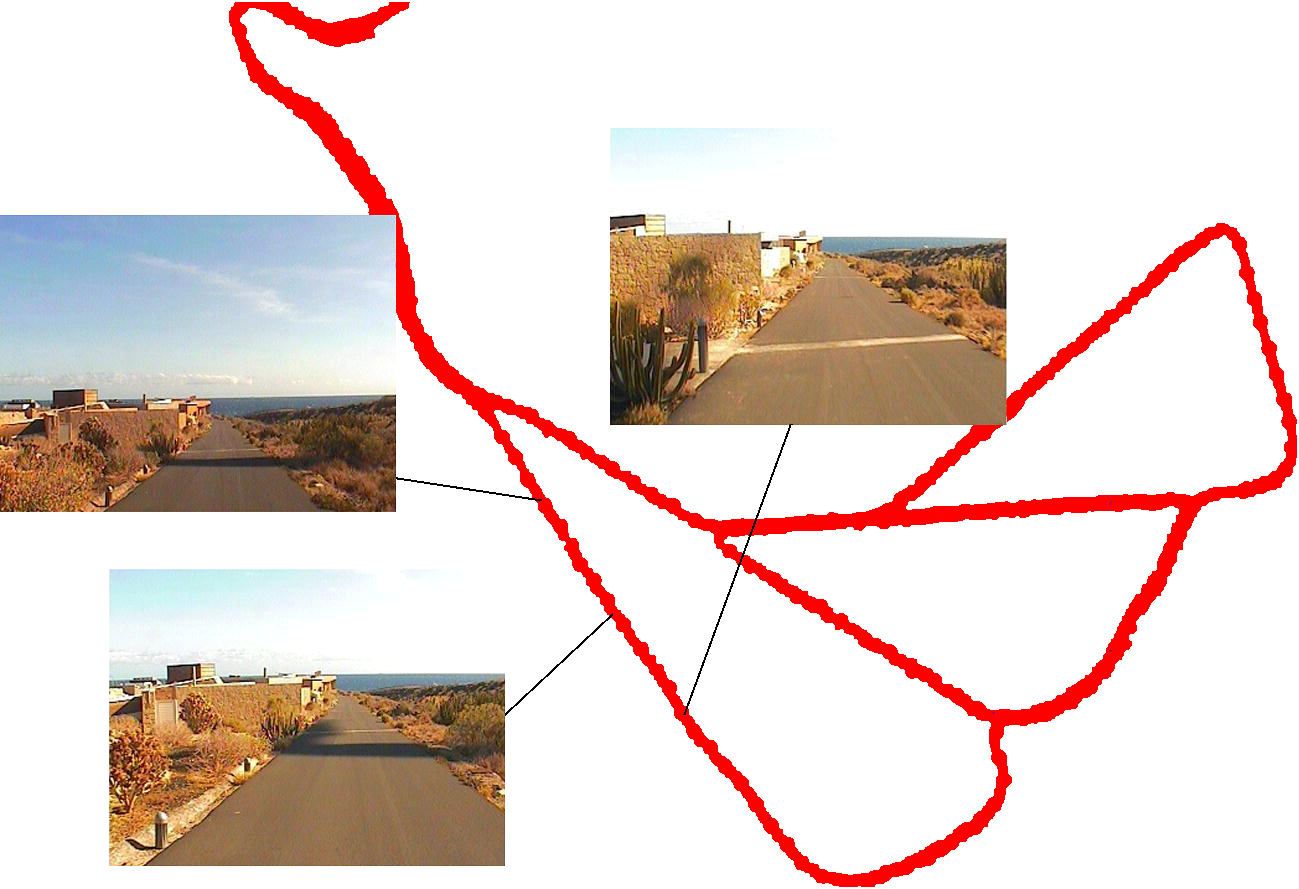
\includegraphics{database}
  \end{center}
  
  \note {
  the vehicle will travel inside the covered area, driven by a human or in controlled conditions. While the vehicle is driven, the system stores the set of $320 \times 240$ images, associating geographic information to them: \emph{latitude}, \emph{longitude}, \emph{height} and their transformation into $x$, $y$, $z$ and orientation coordinates with respect to the coordinates frame of the local map. Other information that could be outstanding in the future is also stored (i.e., the day and the hour in which the image was taken, \acs{GPS} rms value, etc.). Images are preprocessed to have as much information as possible, reducing the execution times. For example, we get the set of features from the images offline, not in the real time application. With a $5\,Hz$ update rate, an image is stored about each traveled meter, depending on the speed of the vehicle. In this phase, there should not be any obstacle in the road where the car is going to drive.
  In real time, the vehicle starts driving by itself. Along the path, it passes over different positions near the recorded route. Positions reported by the \acs{GPS} device are transformed into local coordinates. Simultaneously, an image is obtained from the camera while the nearest image in the database is retrieved. The current frame $I_{RT}$ and the image retrieved from the database $I_{DB}$ are compared by using image change detection techniques, obtaining the obstacles in the scene.
  }
\end{frame}

\begin{frame}{Image registration}
  \begin{enumerate}
    \item Feature detection
    \item Feature matching
    \item Transform model estimation
    \item Image resampling and transformation
  \end{enumerate}

  \note {
  
  }
\end{frame}

\begin{frame}{Image registration - Feature detection}
  Several feature detection methods considered:
  \begin{itemize}
    \item \cite{harris1988combined} / \cite{shi1994good}\\
    \begin{center}
      \begin{figure}[h!]
	\centering
	\begin{subfigure}[b]{0.45\textwidth}
		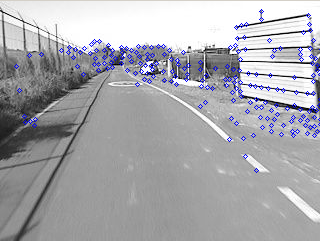
\includegraphics[height=0.3\textheight]{featuresShi1}
	\end{subfigure}%        
	~
	\begin{subfigure}[b]{0.45\textwidth}
		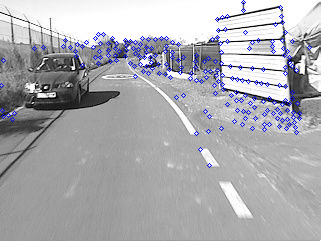
\includegraphics[height=0.3\textheight]{featuresShi2}
	\end{subfigure}%
      \end{figure}
    \end{center}
    \item SIFT \citep{lowe1999object}, SURF \citep{bay2008speeded}\\
    \begin{center}
      \begin{figure}[h!]
	\centering
	\begin{subfigure}[b]{0.45\textwidth}
		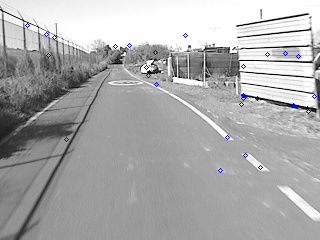
\includegraphics[height=0.3\textheight]{featuresSIFT1}
	\end{subfigure}%        
	~
	\begin{subfigure}[b]{0.45\textwidth}
		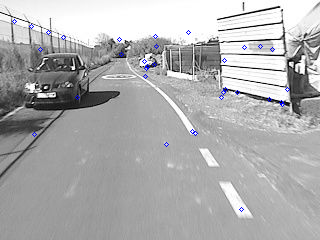
\includegraphics[height=0.3\textheight]{featuresSIFT2}
	\end{subfigure}%
      \end{figure}
    \end{center}
  \end{itemize}

  \note {
  
  }
\end{frame}

\begin{frame}{Image registration - Feature matching}
  \begin{center}
    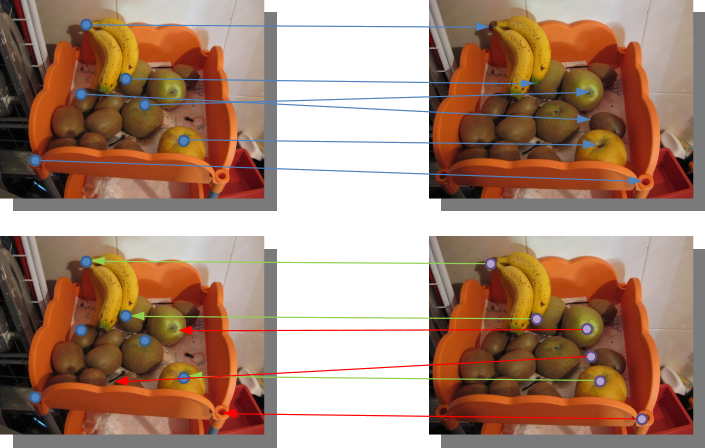
\includegraphics[width=\textwidth]{oFlowMatching}
  \end{center}

  \note {
  
  }
\end{frame}

\begin{frame}{Image registration - Feature matching}
  \begin{center}
      \begin{figure}[h!]
	\begin{subfigure}[b]{0.45\textwidth}
		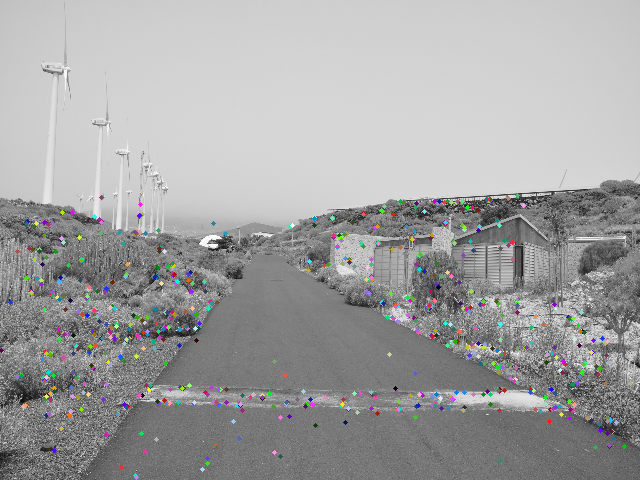
\includegraphics[width=\textwidth]{matches1}
	\end{subfigure}%        
	~
	\begin{subfigure}[b]{0.45\textwidth}
		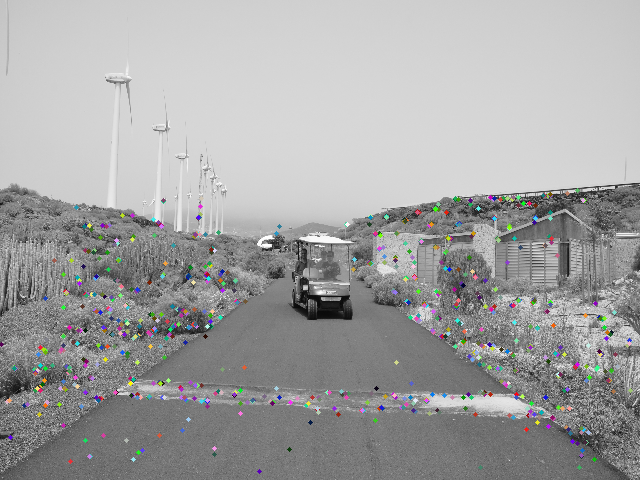
\includegraphics[width=\textwidth]{matches2}
	\end{subfigure}%
      \end{figure}
    \end{center}

  \note {
  
  }
\end{frame}

\begin{frame}{Image registration - Transform model estimation}
  \begin{itemize}
    \scriptsize
    \item Thin-Plate Splines (TPS) \citep{harder1972interpolation} $\rightarrow \mathcal{O}(N^2) + \mathcal{O}(n^2N)$
    \item Weighted Mean (WM) \citep{goshtasby1993design} $\rightarrow \mathcal{O}(n^2N)$
    \item Piecewise Linear (PL) \citep{goshtasby1986piecewise} $\rightarrow \mathcal{O}(N~log(N)) + \mathcal{O}(n^2)$
  \end{itemize}

  \begin{center}
    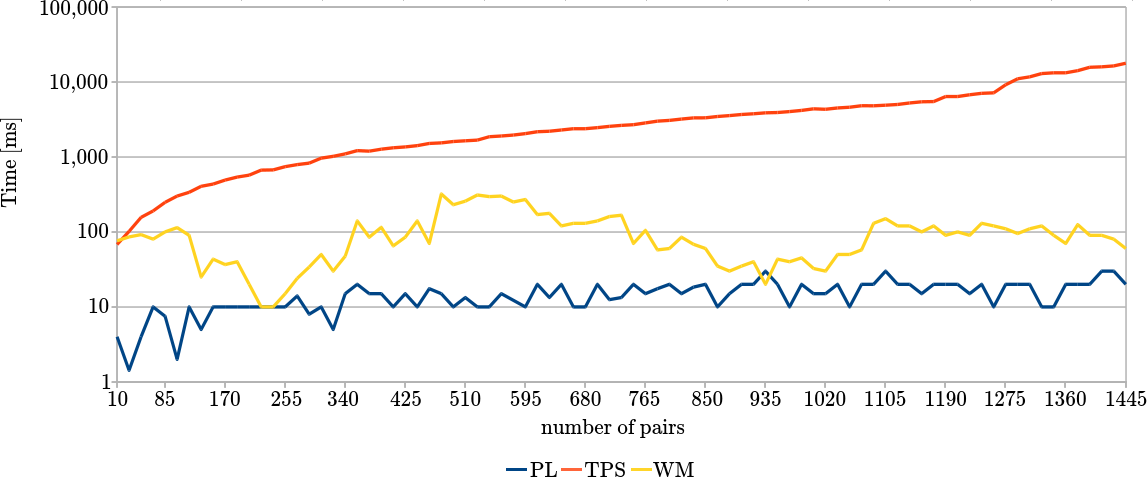
\includegraphics[width=\textwidth]{compTransf}
  \end{center}

  \note {
  
  }
\end{frame}

\begin{frame}{Image registration - Piecewise Linear Transformation}
  \begin{figure}[h!]
    \centering
    \begin{subfigure}[b]{0.3\textwidth}
	    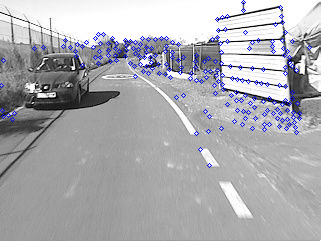
\includegraphics[width=\textwidth]{triangulation1}
    \end{subfigure}%        
    ~
    \begin{subfigure}[b]{0.3\textwidth}
	    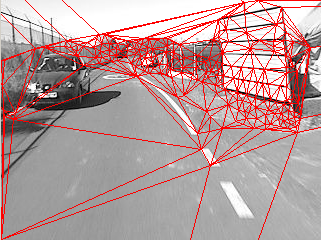
\includegraphics[width=\textwidth]{triangulation2}
    \end{subfigure}%
    \\~\\~
    \begin{subfigure}[b]{0.3\textwidth}
	    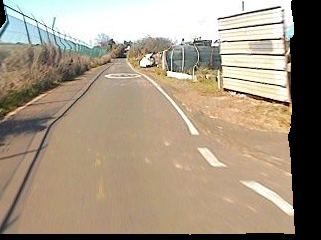
\includegraphics[width=\textwidth]{transformed}
    \end{subfigure}%
  \end{figure}
\end{frame}

\begin{frame}{Obstacle detection}
  \begin{enumerate}
    \item<1-> Mask generation
    \item<2-> Obstacle detection
    \item<3-> Selection of the desired obstacles
  \end{enumerate}

  \begin{overlayarea}{\textwidth}{0.5\textheight}
    \only<1>{
      \begin{figure}
	  \centering
	  \begin{subfigure}[b]{0.3\textwidth}
	    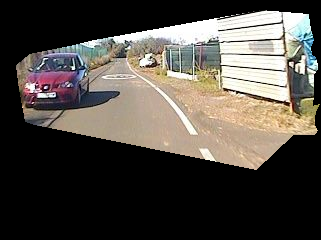
\includegraphics[width=\textwidth]{maskCovers2}
	  \end{subfigure}%        
	  ~
	  \begin{subfigure}[b]{0.3\textwidth}
	    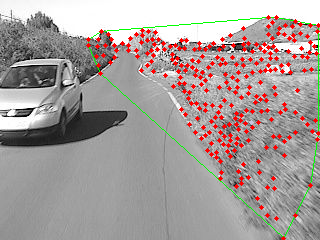
\includegraphics[width=\textwidth]{maskNotCovers}
	  \end{subfigure}%
      \end{figure}
    }
    \only<2>{
      \begin{figure}
	\centering
	\begin{minipage}{0.3\textwidth}
	  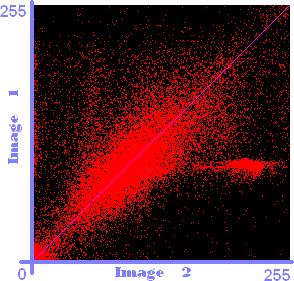
\includegraphics[width=\textwidth]{pca1}
	\end{minipage}
	\begin{minipage}{0.3\textwidth}
	    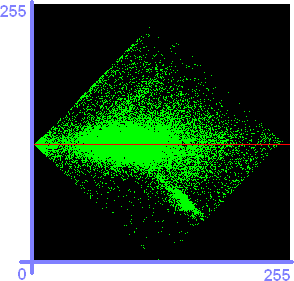
\includegraphics[width=\textwidth]{pca2}
	\end{minipage}
	\begin{minipage}{0.3\textwidth}
	  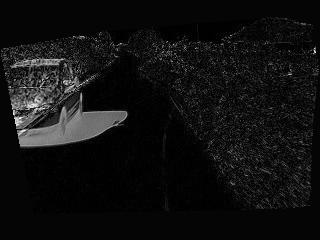
\includegraphics[width=\textwidth]{pca3}
	\end{minipage}
      \end{figure}
    }
    \begin{center}
      \includegraphics<3>[width=0.3\textwidth]{maskWarped}
    \end{center}
  \end{overlayarea}
\end{frame}

\begin{frame}{Obstacle detection}
  \begin{figure}[t]
	\centering
	\begin{subfigure}[b]{0.24\columnwidth}
	    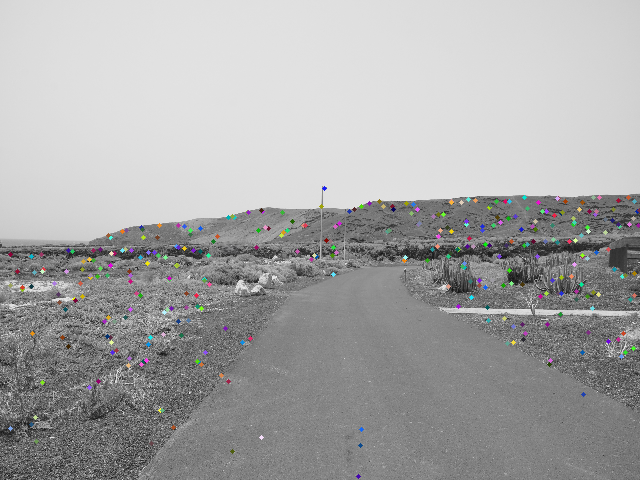
\includegraphics[width=\textwidth]{pipeline/fig5}\label{fig:pipelineA_1}
	\end{subfigure}% 
	~
	\begin{subfigure}[b]{0.24\columnwidth}
	    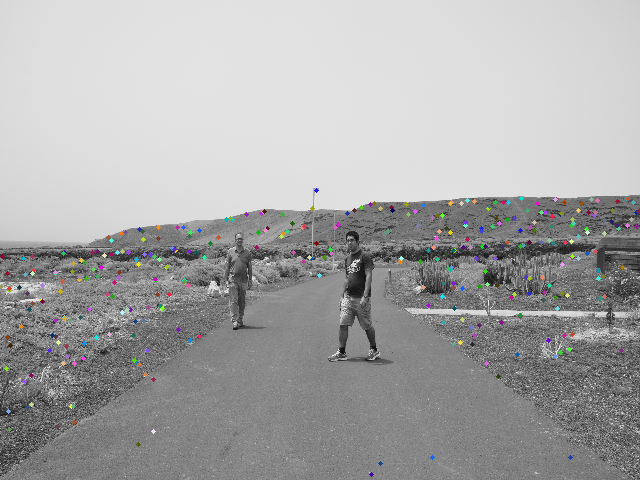
\includegraphics[width=\textwidth]{pipeline/fig4}\label{fig:pipelineA_2}
	\end{subfigure}%       
	~
	\begin{subfigure}[b]{0.24\columnwidth}
	    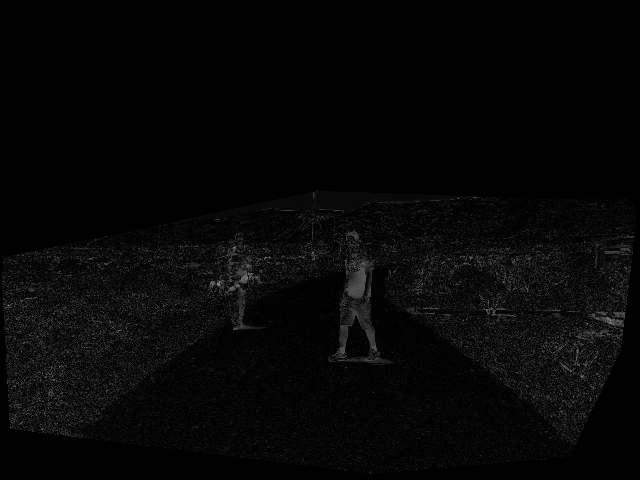
\includegraphics[width=\textwidth]{pipeline/fig2}\label{fig:pipelineA_3}
	\end{subfigure}%    
	~
	\begin{subfigure}[b]{0.24\columnwidth}
	    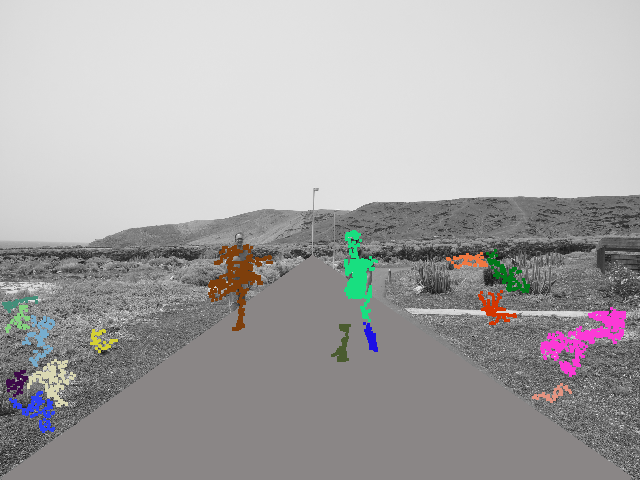
\includegraphics[width=\textwidth]{pipeline/fig3}\label{fig:pipelineA_4}
	\end{subfigure}%
	\\
	\begin{subfigure}[b]{0.24\columnwidth}
	    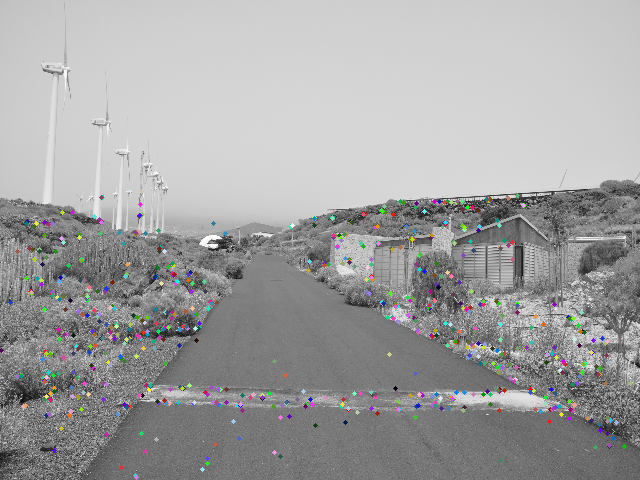
\includegraphics[width=\textwidth]{pipeline2/fig2}\label{fig:pipelineB_1}
	\end{subfigure}% 
	~
	\begin{subfigure}[b]{0.24\columnwidth}
	    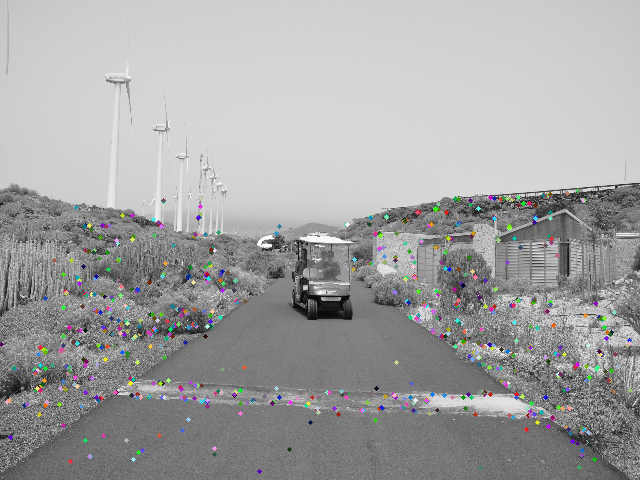
\includegraphics[width=\textwidth]{pipeline2/fig1}\label{fig:pipelineB_2}
	\end{subfigure}%       
	~
	\begin{subfigure}[b]{0.24\columnwidth}
	    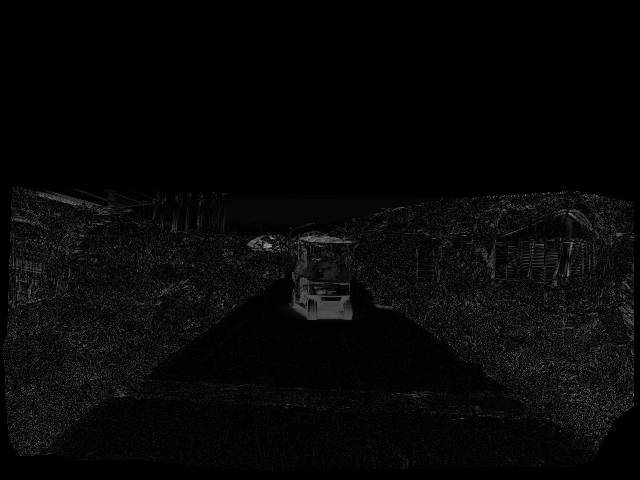
\includegraphics[width=\textwidth]{pipeline2/fig4}\label{fig:pipelineB_3}
	\end{subfigure}%    
	~
	\begin{subfigure}[b]{0.24\columnwidth}
	    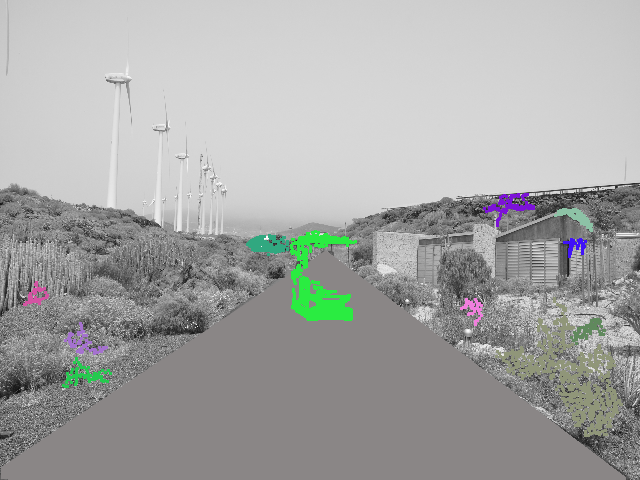
\includegraphics[width=\textwidth]{pipeline2/fig5}\label{fig:pipelineB_4}
	\end{subfigure}%
  \end{figure}
\end{frame}

\begin{frame}{Obstacle detection and tracking}
  \begin{itemize}
  \item Goals:
    \begin{enumerate}
    \item Good obstacle detection rate. \only<2->{\textcolor{green}{\cmark}}
    \item Obstacle localization. \only<7->{\textcolor{red}{\xmark}}
    \item Real time. \only<3->{\textcolor{green}{\cmark}}
    \item Environment conditions independence. \only<6->{\textcolor{red}{\xmark}}
    \item Tracking capabilities. \only<5->{\textcolor{red}{\xmark}}
    \item Moving cameras. \only<4->{\textcolor{green}{\cmark}}
    \end{enumerate}
  \end{itemize}
\end{frame}